\renewcommand*{\arraystretch}{1.1}

\noindent\begin{tabularx}{17cm}{|p{1.95cm}|X|}
	\hline
	workload    & BI \\ \hline
%
	query       & 17 \\ \hline
%
	title       & Friend triangles \\ \hline
	\multicolumn{2}{|c|}{ 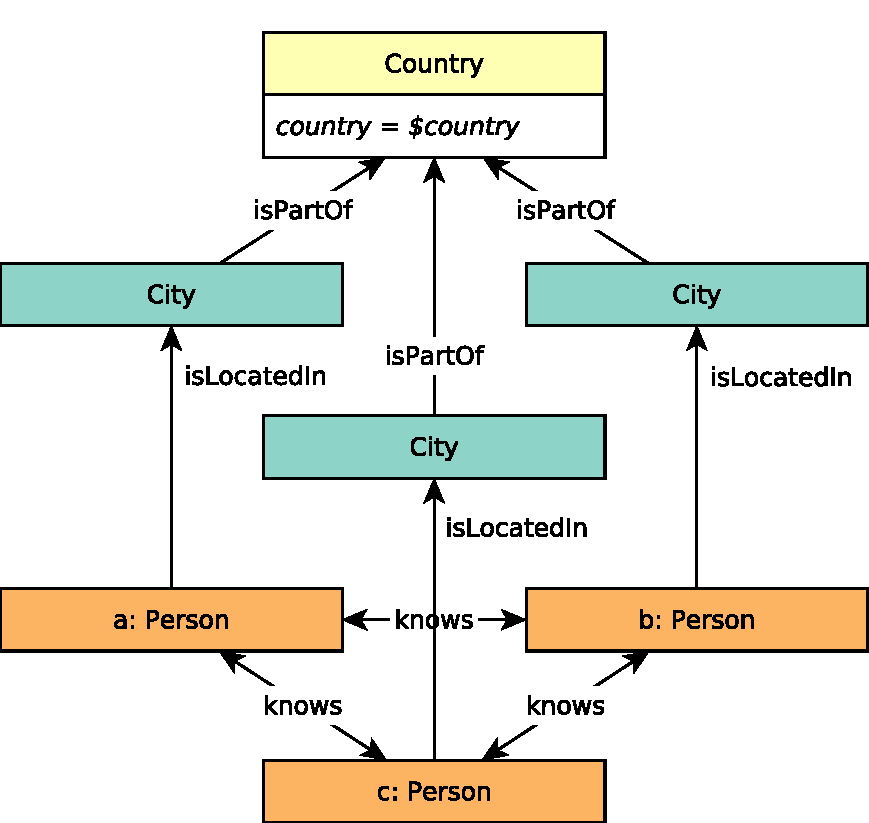
\includegraphics[scale=\patternscale,margin=0cm .2cm]{patterns/bi17}} \\ \hline
	description & For a given country, count all the distinct triples of persons such that
\texttt{a} is friend of \texttt{b}, \texttt{b} is friend of \texttt{c},
and \texttt{c} is friend of \texttt{a}.

Distinct means that given a triple \(t_1\) in the result set \(R\) of
all qualified triples, there is not a triple \(t_2\) in \(R\) such that
\(| t_1 \cup b | = 3\).
 \\ \hline
	
%
	parameters  &
	\vspace{1.1ex}{\begin{tabularx}{14.38cm}{|c|M|m{2cm}|Y} \hline
	\cellcolor{black!70} \color{white} $\mathsf{1}$ & \varname{country} & \cellcolor{gray!20} \vartype{String} &  \\
	\end{tabularx}} \\ \hline
%
	result      &
	\vspace{1.1ex}{\begin{tabularx}{14.38cm}{|c|M|m{2cm}|Y} \hline
	\cellcolor{black!70} \color{white} $\mathsf{1}$ & \varname{count} & \cellcolor{gray!20} \vartype{32-bit Integer} &  \\
	\end{tabularx}} \\ \hline
	%
	%
	choke points &
	\multicolumn{1}{>{\raggedright}X|}{
		\chokepoint{1.1}, 
		\chokepoint{2.3}
		}\\ \hline
\end{tabularx}
\clearpage